\documentclass[10pt, letterpaper]{article}

% Preamble
\usepackage{url}
\usepackage[
    backend=biber,
    style=alphabetic,
    sorting=ynt
    ]{biblatex}
\addbibresource{../bib/articles.bib}
\addbibresource{../bib/notebooks.bib}

\begin{document}
\section{Overview of Semi-Supervised Learning Litterature}
\subsection{Overview of general models}
\subsubsection{Generative Mixture Models and EM}
This model works by assuming a generative model:
$$
    p(x, y) = p(y)p(x|y)
$$
where $p(x|y)$ is an identifiable mixture distribution such as Gaussion mixture models. The idea is then with a large amount of unlabelled data that the mixture components can be identified, and then ideally only one labelled example per component is needed to fully determine the mixture distribution. A general way of thinking of this is that the mixture components are "soft clusters".



\paragraph{Gaussian distribution}
The gaussian distribution is historically called the law of errors. It was by Gauss to model errors in astromocial observations, which is why it is usually refered to as the Gaussian distribution. The formula for the Gaussian distribution given mean $\mu$ and standard deviation $\sigma$ is given by:
$$
    \phi(x; \mu, \sigma) = \frac{1}{\sigma \sqrt{2 \pi}} \exp{-\frac{(x-\mu)^2}{2\sigma^2}}
$$

An important concept within mixture models in general is identifiability. In general let $\{p_\theta\}$ be a family of distributions indexed by a parameter vector $\theta$. $\theta$ is identifiable if $\theta_1 \neq \theta_2 \Rightarrow p_{\theta_0} \neq p_{\theta_1}$. If the model family is identifiable, in theory with infinite $U$ one can learn $\theta$ up to permutation of component indices.\\
In contrast an example where the problem of an unindetiable is shown. Given a model $p(x|y)$ that is uniform for

\section{Convergence}
Convergence in the context of Machine Learning when the training-validation error is so close to local/global minimum or you can see it having a perfomance so close to local/global minimum that usually no significant error decrease/increase in perfomance anymore.

\section{Semi-Supervised Learning}
A recurring problem in data science is the lack of labels in data sets\cite{zhusurvey}. This problem is often due to either the expense of labeling due to the requirement of having a human classifying the images or the immensity of the data set, making the task of labeling long if not endless. Semi-supervised learning is used as an answer to this problem under some conditions. In essence, SSL is in most cases a unique form of classification. SSL can also be used for clustering, but as this thesis only used classification, this will not be explored further.\\ 
Traditionally when classifying, one would need a data set with labels as a feature-label pair and use supervised learning to solve the problem or have a data set with no labels to cluster in unsupervised learning. Semi-supervised learning addressed this gap in Machine Learning of label sparsity by coupling labeled and unlabelled data and making better classifiers, i.e., relabelling the unlabelled data set, with the assumption that there is some correlation between the labeled and the unlabelled data, i.e., if a data point in the labeled data set is similar to a data point in the unlabelled data set, there is some probability that these bear the same label. 



\subsection{Assumptions}
Semi-Supervised learning works under some assumptions as not all problems can be solved with SSL.  In that case, we analyze the data and can see from the known labeled data that there is some coherence between features and labels, or we visualize and see that we get some nice clusters that make sense, we can be reasonably sure that the method will yield better classifiers than the previous dataset. If, on the other hand, the data is very "messy," we can probably assume that the dataset is too "dense" or cluttered, and the semi-supervised learning approach might be a bad idea. To get a better visual understanding of this, please look at \Cref{fig:meth-circles}.

\begin{figure}[!ht]
    \centering
    \begin{subfigure}[t]{.45\linewidth}
      \centering
      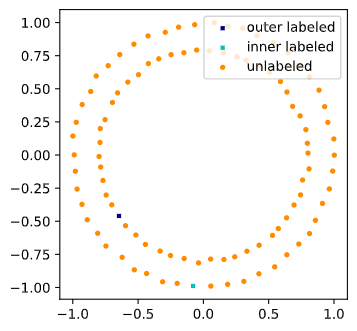
\includegraphics[width=.8\linewidth]{Pictures/Methods/SSL/circle_low_noise_3.png}
      \caption{Low noise}
      \label{fig:meth-lownoise}
    \end{subfigure}
    \hfill
    \begin{subfigure}[t]{.45\linewidth}
      \centering
      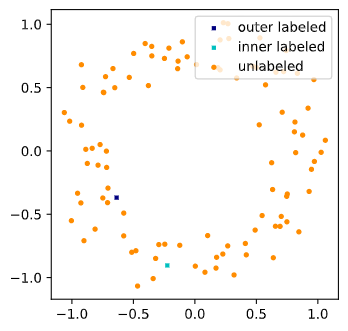
\includegraphics[width=.8\linewidth]{Pictures/Methods/SSL/circle_high_noise_3.png}
      \caption{High noise}
      \label{fig:meth-highnoise}
    \end{subfigure}
    \caption{Random circles made with \href{https://scikit-learn.org/stable/modules/generated/sklearn.datasets.make\_circles.html}{sklearn.datasets.make\_circles}. Example illustrates dataset with only one known label in each circle. There is a nice correlation between label and circle in \cref{fig:meth-lownoise} and self training would be able to nicely classify the two circle, but if the noise increases the distinction between outer and inner circle becomes too undefined to make any qualified guesses}
    \label{fig:meth-circles}
\end{figure}

Using some intuition when looking at \cref{fig:meth-lownoise} and \cref{fig:meth-highnoise}, we see the probability of making accurate classifiers to be much higher in \cref{fig:meth-lownoise} simply because there is a distance between the inner and outer circle, while looking at \cref{fig:meth-highnoise} one might expect that the data instead of getting separated into two circles gets labeled as a left/up cluster, and a down/right cluster. The question of bad matching does remain an open problem, and will have to be identified on a per data set basis \cite{zhusurvey}.

\newpage
\nocite{*}
\printbibliography[heading=bibintoc,title={Bibliography}]


\end{document}